\chapter{Visualisation implementation}\label{C:sd}
This section details the implementation of the Improved Kepler Visualisation Tool. It details decisions that were made during the project such as choosing a viable framework, the choice of extending a previous system, and  platform choice.   
\section{Technology choice}
Many technologies were looked into,experimented with, and the positives and negatives of each weighed up before a decision was made about which would be the choice for the visualisation. 

\subsubsection{D3 (Data Driven Documents)}
D3 is a JavaScript library that allows the displaying of data in dynamic graphics. Embedded
within an HTML web page, the JavaScript D3.js library uses pre-built JavaScript functions to
select elements, create Scalable Vector Graphic (SVG)[17] objects, style them, and add transitions,
dynamic effects and tooltips. Large datasets can be easily bound to SVG objects using
simple D3 functions to generate rich charts and diagrams. D3 was created because of the
need for a balance of expressiveness, efficiency, and accessibility that previous visualization
toolkits did not allow [4].

D3 allows the binding of input data to arbitrary input elements. This means that the exoplanet
dataset can easily be bound to SVG elements for creating visualizations. D3 adopts
the W3C Selectors API to identify document elements queried. This results in a rich but
concise selection method of elements in a visualisation.

D3 allows debugging thanks to Google chrome and other modern browsers development
tools. A downside to D3 is that it does not allow 3D diagrams, although it does allow
pseudo 3D by using the painter’s algorithm and textures.

\subsubsection{Prefuse}
Prefuse is a set of software tools for creating rich interactive data visualizations [13]. The
Prefuse toolkit provides a visualization framework for Java. It supports a set of features
for visualizing and interacting with data. It provides optimized data structures for tables,
graphs, and trees. It can be used to build standalone applications, visual components embedded
in larger applications, and web applets. Prefuse to greatly simplifies the process
of representing and efficiently handling data, mapping data to visual representations (e.g.,
through spatial position, size, shape, color, etc), and interacting with the data.
To use Prefuse a basic familiarity with the Java is required, including setting up and building
Java projects. A knowledge of Swing or another similar user interface toolkit is also
useful for understanding some of the concepts behind Prefuse and for integrating Prefuse
visualizations into larger applications. Experience with database systems is also helpful. 
However the complexity of Prefuse means that the learning curve will be out of scope for
this project.

\subsubsection{Processing}
Processing is an open source programming
language and development environment that was initially created to serve as a software
sketchbook and to teach the fundamentals of computer programming with a visual context.
Using processing would mean that the visualization could be built with Java while still using
a successful visualisation framework. The most complete existing visualization using
the same exoplanet dataset (Kepler Visualization Tool) is built using Processing .
Using this solution would involve learning the Processing language, however Processing
is a library built in Java so the syntax is the same. This means the learning curve in in regards
to the program itself should be shallow.
\\
Using processing and would mean that 3D elements could be included, this wouldnt be
possible with D3. However it does require a strong knowledge in 3D transformations which
I do not possess. This may be a limiting factor in the speed at which I could understand the
existing code and may push using this solution out of scope in favor of D3.

\clearpage
\begin{figure}[h!]
  \centering
      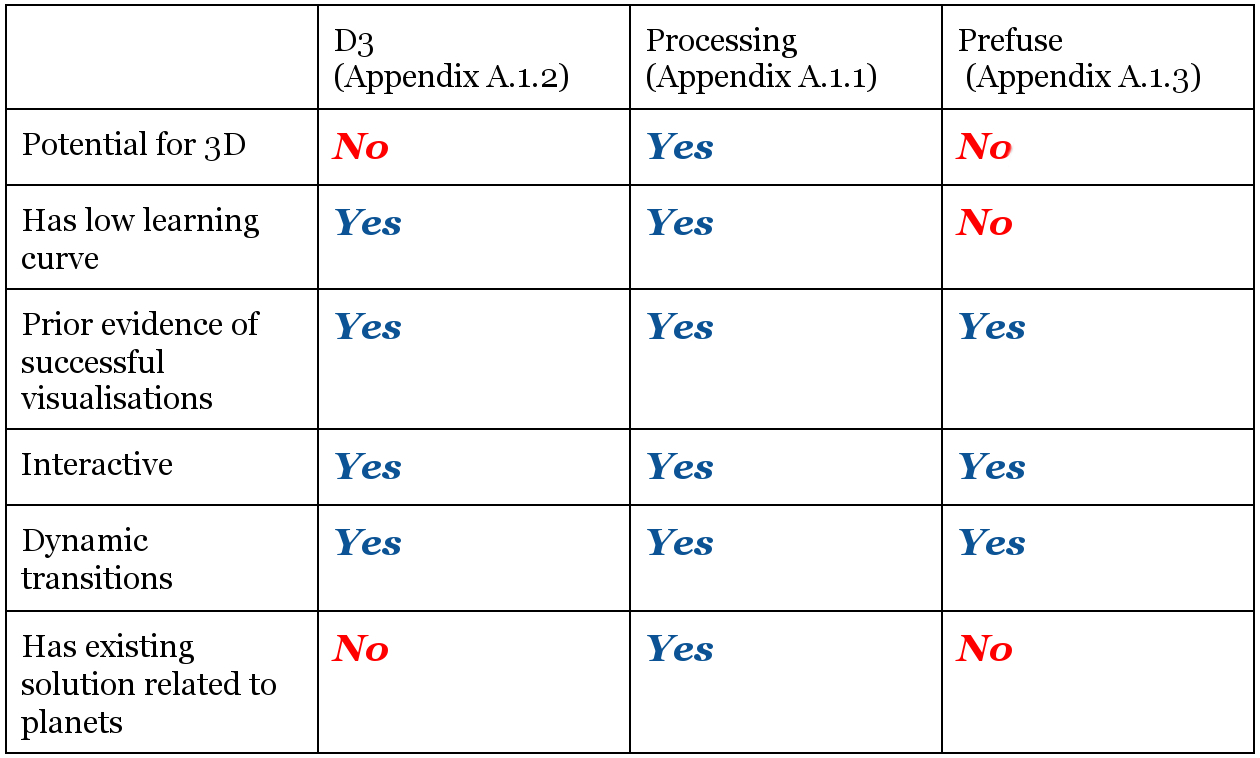
\includegraphics[width=0.8\textwidth]{images/table_technologies.jpg}
  \caption{Table of technology choices}
\end{figure}


\subsection{System design and structure}

\subsection{Tools and artifacts used}
\section{Extension to initial design}


